\documentclass{article}
\usepackage{tikz, comment}
\usepackage{pifont}
\usepackage{fontspec}
\usetikzlibrary{arrows, decorations.markings, decorations.pathreplacing}
\begin{comment}
:Title: Not defined yet
:Tags: aa similarity;aas congruence, saa congruence ;abscissa;absolute convergence, absolutely convergent ;absolute maximum, absolute max, global maximum, global max
:Prob: nan;nan;nan;nan;nan
:Author: Prof.Hu Ji-shan, HKUST
:Slug: No name yet

Description Here.........
\end{comment}
\begin{document}\centering

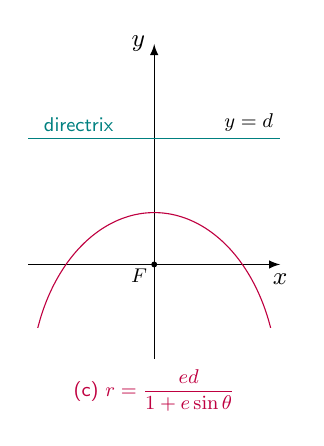
\begin{tikzpicture}[>=latex,xscale=.5*0.4, yscale=.5*0.4][font=\sf\small]

\draw[->] (-8, 0) -- (8, 0)node[below] {\small $x$};
\draw[->] (0, -6) -- (0, 14)node[left] {\small $y$};

\node[purple, scale=0.8] at (0, -8) {(c) $\displaystyle r = \frac{ed}{1+e\sin \theta}$};

\clip[] (-8,-4) rectangle (8, 14.2);

\draw[purple, samples=100, smooth, domain=-pi/2-0.5:pi+0.5, variable=\t]
plot ({0.7*8/(1+0.7*sin(\t r))*cos(\t r)}, {0.7*8/(1+0.7*sin(\t r))*sin(\t r)}) ;

\draw[teal] (-8, 8) -- (8, 8) node[above, pos=0.2, scale=0.8] {$\hbox{directrix}$};

\draw[fill, xscale=1/0.4, yscale=1/0.4] (0, 0) circle(0.06) node[left, yshift=-4, scale=0.8]{$F$};

\node[above, scale=0.8] at (6, 8) {$y=d$};

\end{tikzpicture}\hskip1cm
\end{document}